\documentclass[border=4pt]{standalone}
\usepackage{tikz}
\usetikzlibrary{arrows,arrows.spaced}
\begin{document}
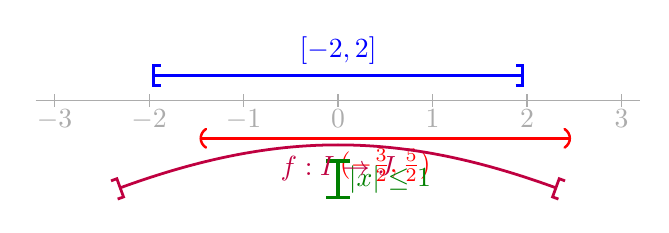
\begin{tikzpicture}[x=12mm,y=10mm]
  \draw[gray!65] (-3.2,0) -- (3.2,0);
  \foreach \x in {-3,-2,-1,0,1,2,3}
    \draw[gray!65] (\x,-.08) -- (\x,.08) node[below=2pt] {$\x$};

  \draw[blue,line width=1.1pt,arrows={spaced [-spaced ]}]
    (-2,.32) -- node[above] {$[-2,2]$} (2,.32);
  \draw[red,line width=.9pt,arrows={spaced (-spaced )}]
    (-1.5,-.48) -- node[below] {$(-\frac32,\frac52)$} (2.5,-.48);
  \draw[green!50!black,line width=1.25pt,arrows={spaced |-spaced |}]
    (0,-1.3) -- node[right] {$|x|\leq1$} (0,-.7);
  \draw[purple,line width=1pt,arrows={spaced ]-spaced [}]
    (-2.4,-1.15) to[bend left=20] node[below,sloped] {$f:I\to J$} (2.4,-1.15);
\end{tikzpicture}
\end{document}
